\section{Sprint 1} \label{sprint_1}

This section contains the sprint 1 Retrospective, Review and Burndown chart

\subsection{Retrospective}
We mostly did well, the load assigned was appropriate. We ended up finishing most things (85\% of the tasks were completed, and a full depiction of what was done is in the review). As in the end we did not complete any item fully, we should split tasks even more


\subsection{Review}
All the work done is indicated here, with details about completion:
\begin{itemize}
	\item Definition of tests 80\% done: defined a clear guideline for the tests including objectives, testing types, testing method approaches, testing environment and report tracking. So the developers have a clear vision and write efficient test cases. The actual tests are missing, but they should take little time, having the template
	\item Environment setup 100\% done: setup the backend based on microservices approach. Containerization with docker, CI/CD with Github Action, deployment with Render
	\item Architecture description 100\% done: completed documentation based on the microservices setup
	\item API definition 30\% done: API research completed, now the actual implementation of GraphQL APIs is missing
	\item Git strategy: 95\% done: the proposal model is defined. There are still minor inconsistencies between git flow type branches and commit message types which should be dealt with
	\item Product backlog: 99\% done: The textual file and its translation into gitHub milestones are complete and redundant with various versions. The backlog items for sprint 1 items have also been inserted, but the definition of their syntax is still not totally clear and ust be refined for sprint 2
	\item Definition of done: 100\% done: the textual file has been completed and the criteria for done have been decided in accordance with the course’s slides
	\item Burndown chart automation 70\% done: the GitHub part is totally set up, it will be 100\% functional for sprint 2
\end{itemize}

\subsection{Burndown chart}
This is the burndown chart for sprint 1

\begin{figure}[h]
	\centering
	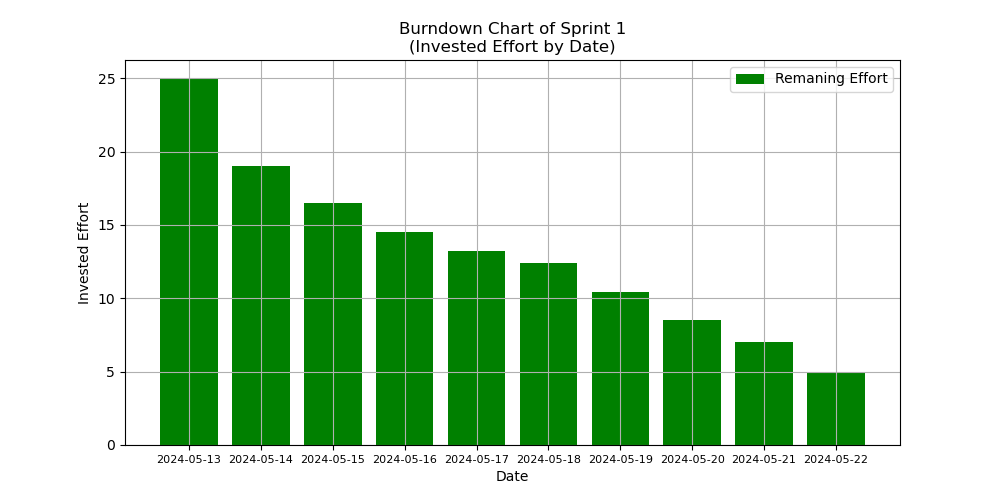
\includegraphics[width=0.9\textwidth]{images/Sprint-1-burndown-chart.png}
\end{figure}

